\section{Task 3/4}

\subsection{Overview of Newton's algorithm}

Newton's divided-difference algorithm interpolates functions. Its main advantage is efficient evaluation of an interpolating polynomial from a given point set. Its \( O(n^2) \) complexity makes it most suitable for moderate input sizes.

Divided differences allow terms to be added incrementally without recomputing the entire polynomial. Tests examined Chebyshev-metric errors at 1000 points with a random sample of $n$ points, assessing how well the fit reproduces the function.

Three functions were tested:
\begin{itemize}
    \item Trigonometric function: \( f(x) = \sin(x) + \cos(x) \),
    \item Rational function: \( f(x) = \frac{1}{1 + x^2} \),
    \item Discontinuous function: \( f(x) = \lfloor x \rfloor \).
\end{itemize}

\subsection{Results and conclusions}

\begin{center}
\textbf{Results for \( \sin(x) + \cos(x) \):}
Minimum error: \( 9.63 \times 10^{-10} \),
achieved with 33 points.
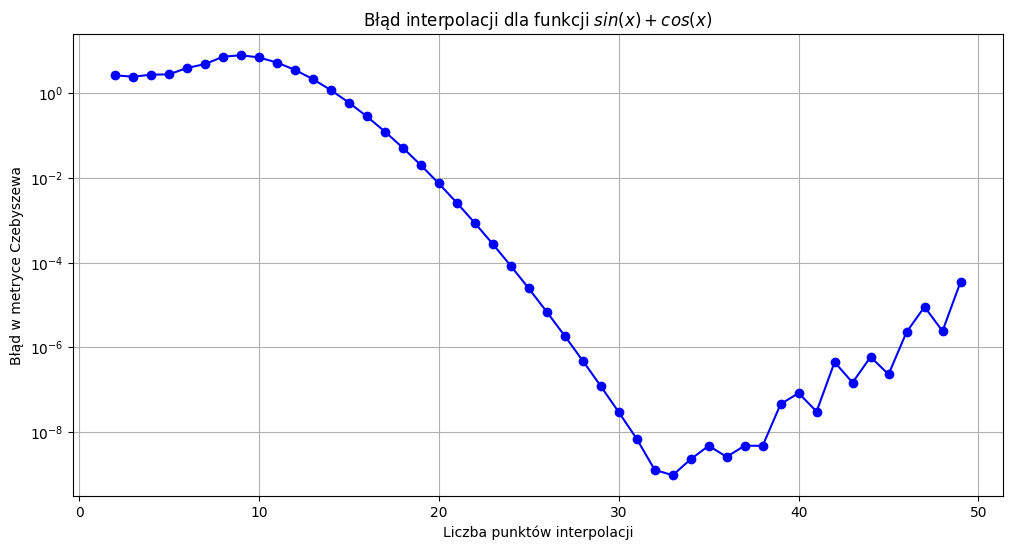
\includegraphics[width=0.8\textwidth]{figures/task-3/trigonometric_error.png}
\end{center}

\begin{minipage}{0.49\textwidth}
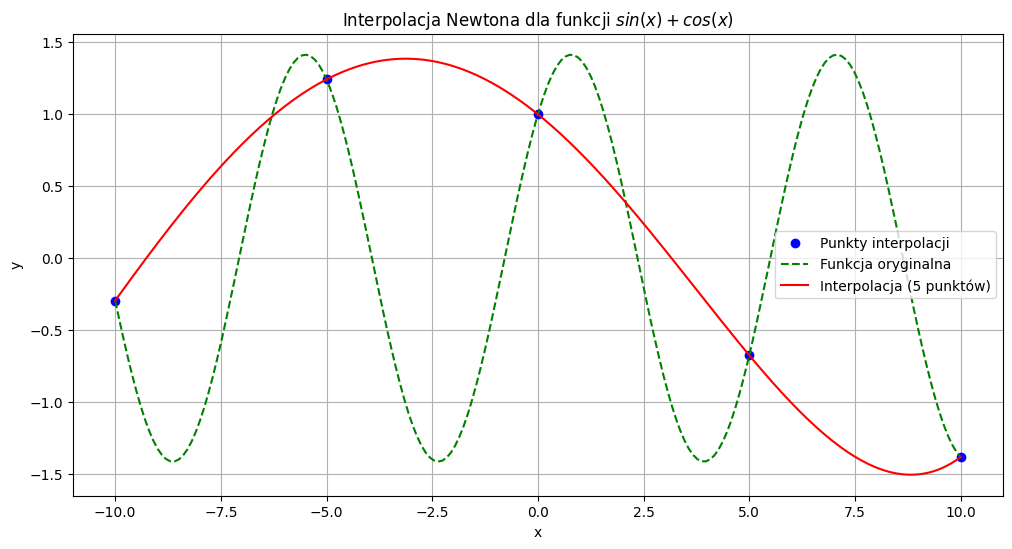
\includegraphics[width=\textwidth]{figures/task-3/trigonometric_5.png}
\end{minipage}
\begin{minipage}{0.49\textwidth}
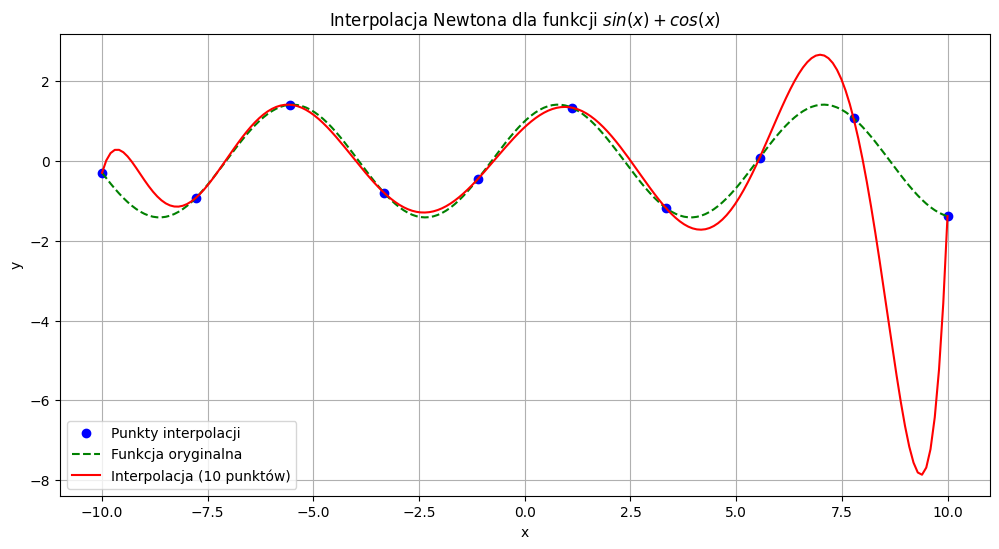
\includegraphics[width=\textwidth]{figures/task-3/trigonometric_10.png}
\end{minipage}

\begin{minipage}{0.49\textwidth}
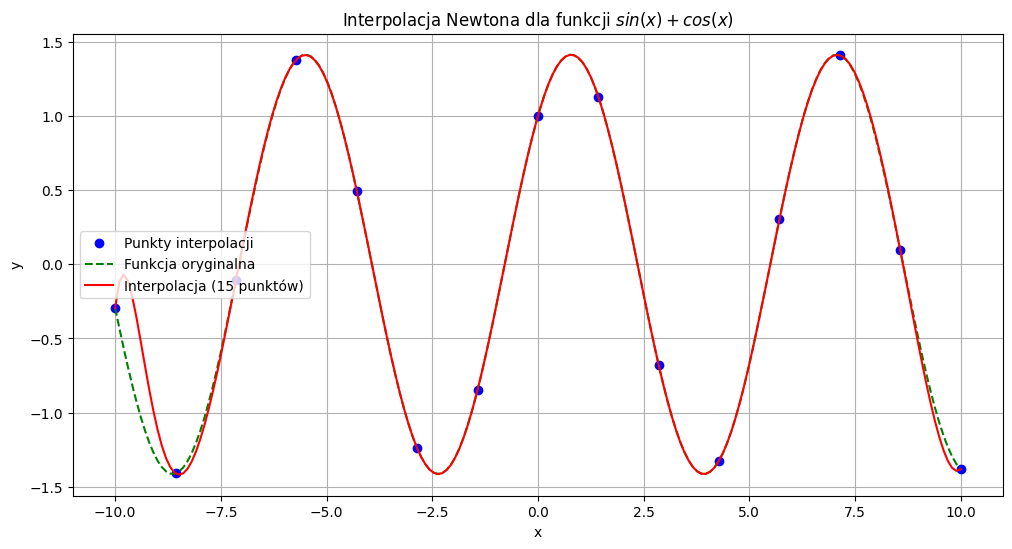
\includegraphics[width=\textwidth]{figures/task-3/trigonometric_15.png}
\end{minipage}
\begin{minipage}{0.49\textwidth}
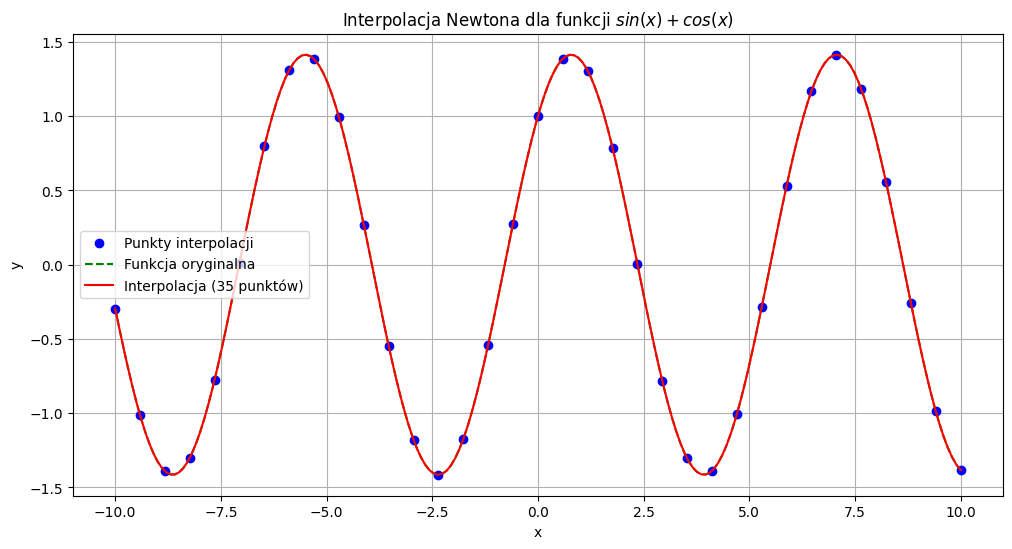
\includegraphics[width=\textwidth]{figures/task-3/trigonometric_35.png}
\end{minipage}

\begin{center}
\textbf{Results for \( \frac{1}{1 + x^2} \):}
Minimum error: \( 4.78 \times 10^{-1} \),
achieved with 10 points.
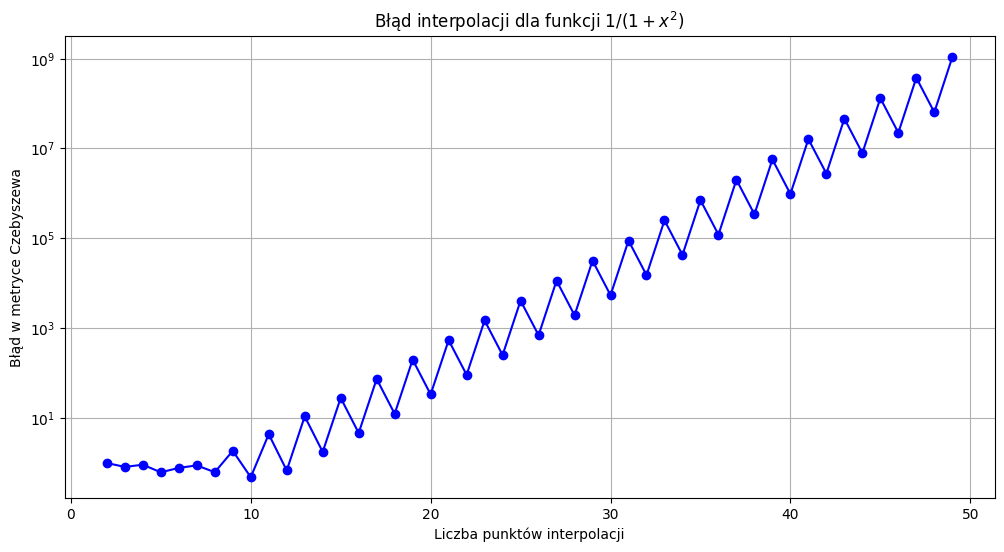
\includegraphics[width=0.8\textwidth]{figures/task-3/rational_error.png}
\end{center}

\begin{minipage}{0.49\textwidth}
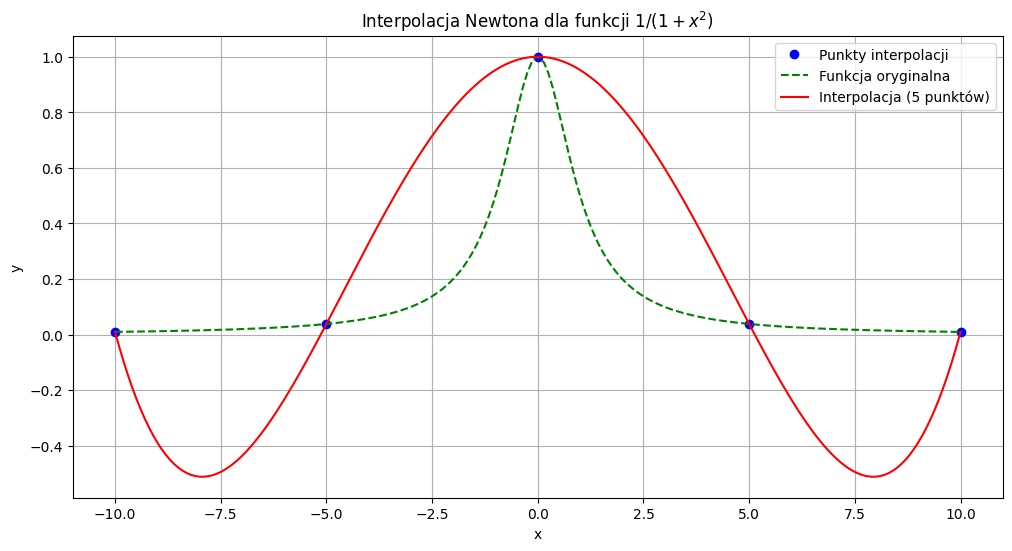
\includegraphics[width=\textwidth]{figures/task-3/rational_5.png}
\end{minipage}
\begin{minipage}{0.49\textwidth}
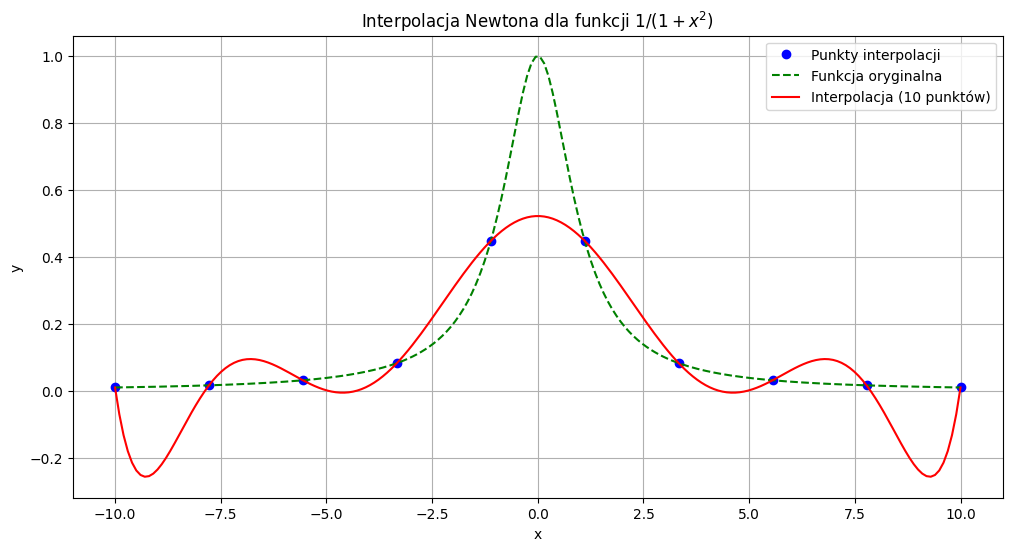
\includegraphics[width=\textwidth]{figures/task-3/rational_10.png}
\end{minipage}

\begin{minipage}{0.49\textwidth}
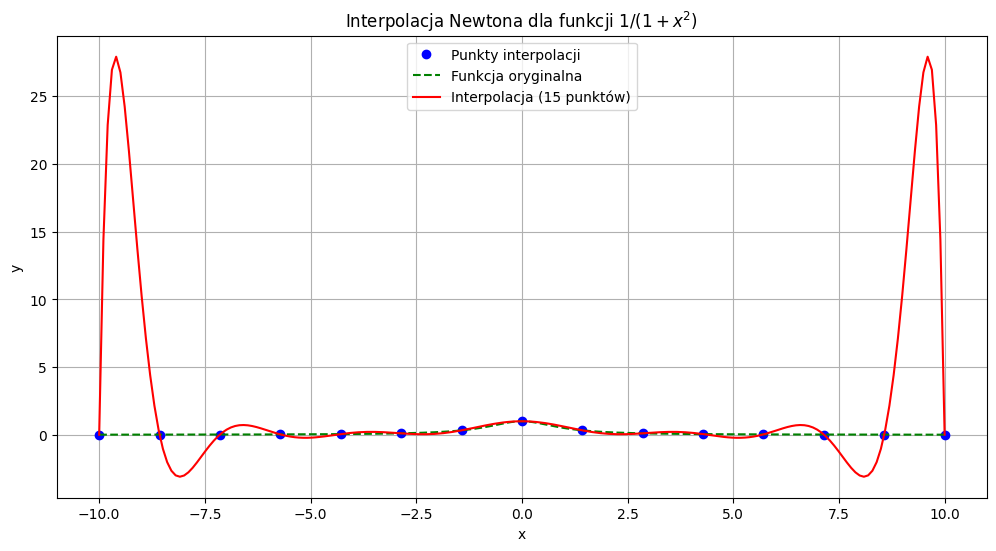
\includegraphics[width=\textwidth]{figures/task-3/rational_15.png}
\end{minipage}
\begin{minipage}{0.49\textwidth}
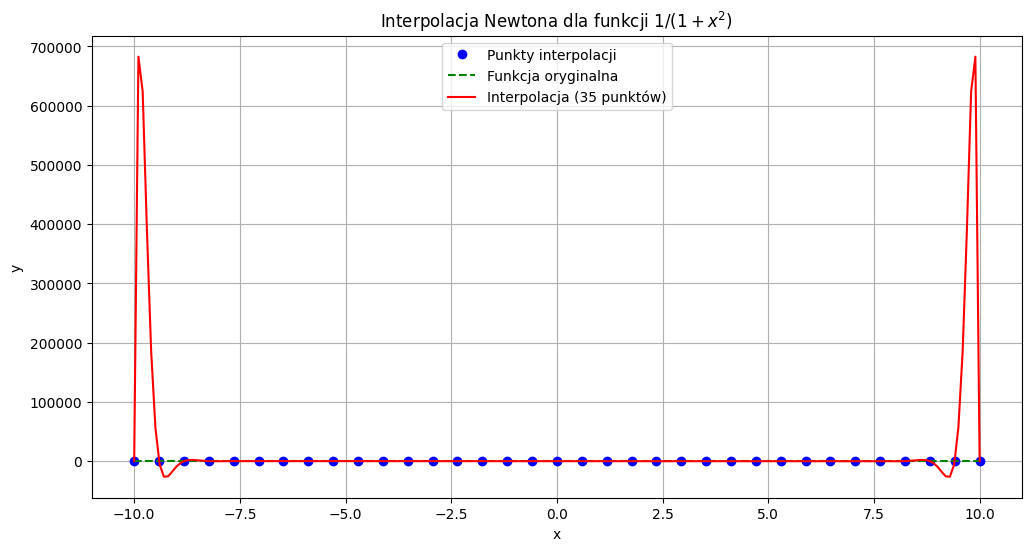
\includegraphics[width=\textwidth]{figures/task-3/rational_35.png}
\end{minipage}

\begin{center}
\textbf{Results for \( \lfloor x \rfloor \):}
Minimum error: \( 9.32 \times 10^{-1} \),
achieved with 20 points.
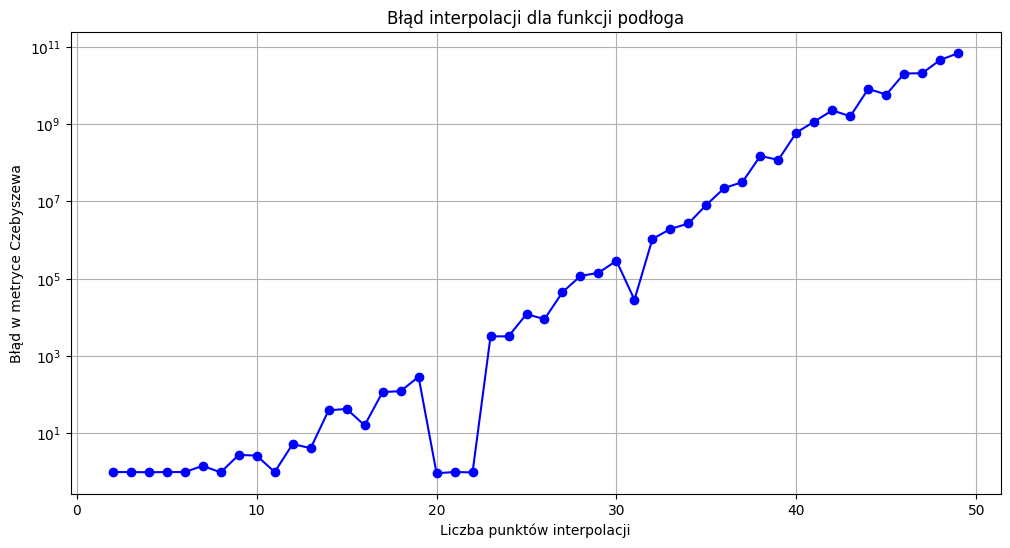
\includegraphics[width=0.8\textwidth]{figures/task-3/floor_error.png}
\end{center}

\begin{minipage}{0.49\textwidth}
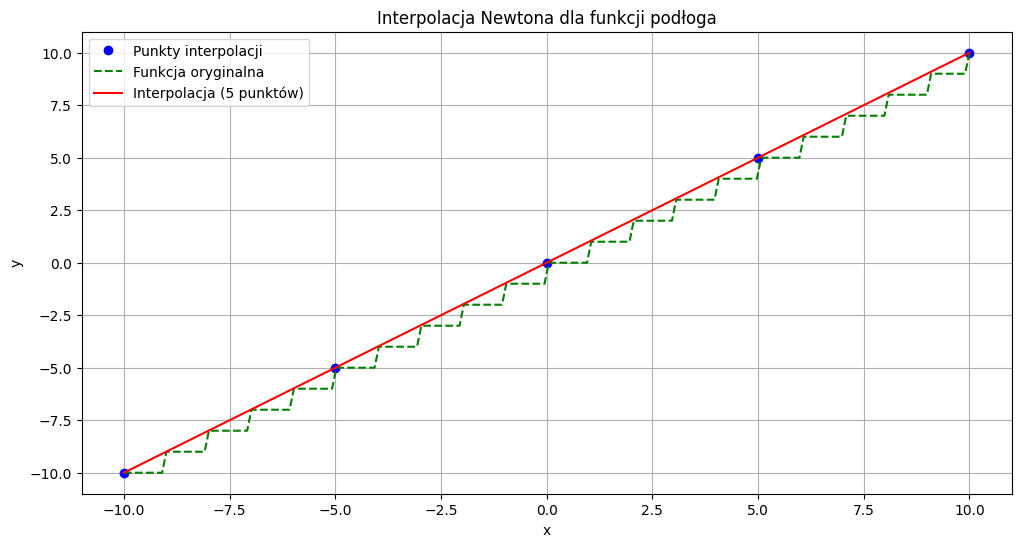
\includegraphics[width=\textwidth]{figures/task-3/floor_5.png}
\end{minipage}
\begin{minipage}{0.49\textwidth}
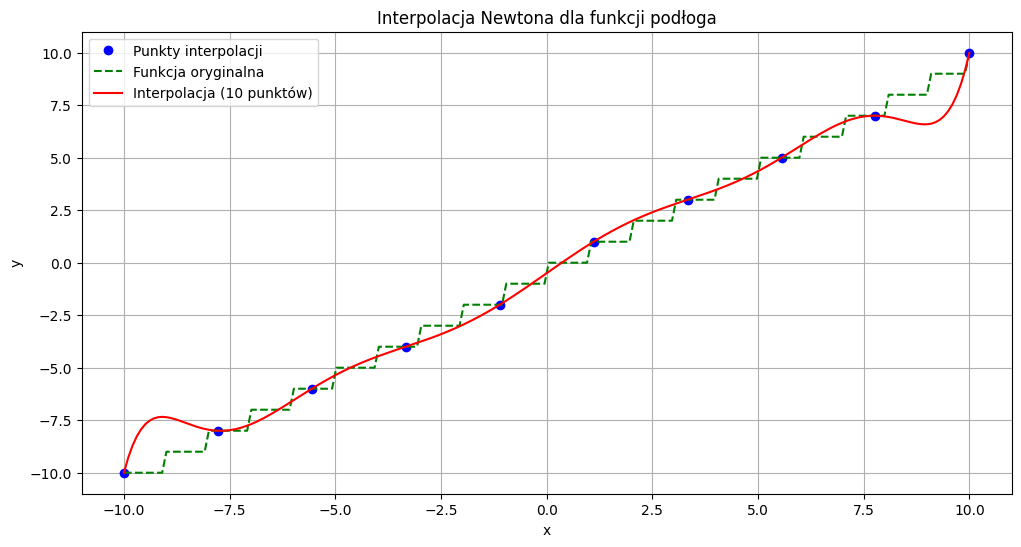
\includegraphics[width=\textwidth]{figures/task-3/floor_10.png}
\end{minipage}

\begin{minipage}{0.49\textwidth}
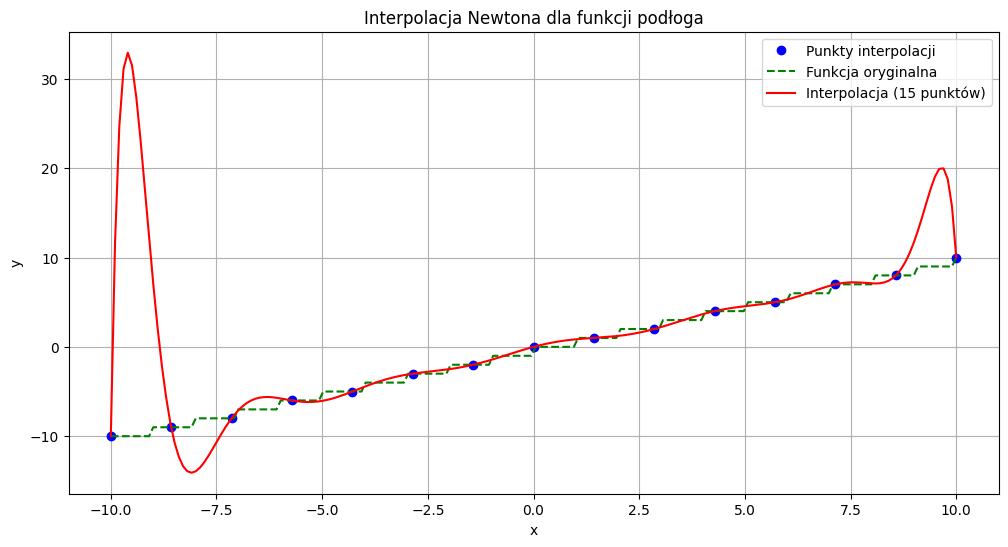
\includegraphics[width=\textwidth]{figures/task-3/floor_15.png}
\end{minipage}
\begin{minipage}{0.49\textwidth}
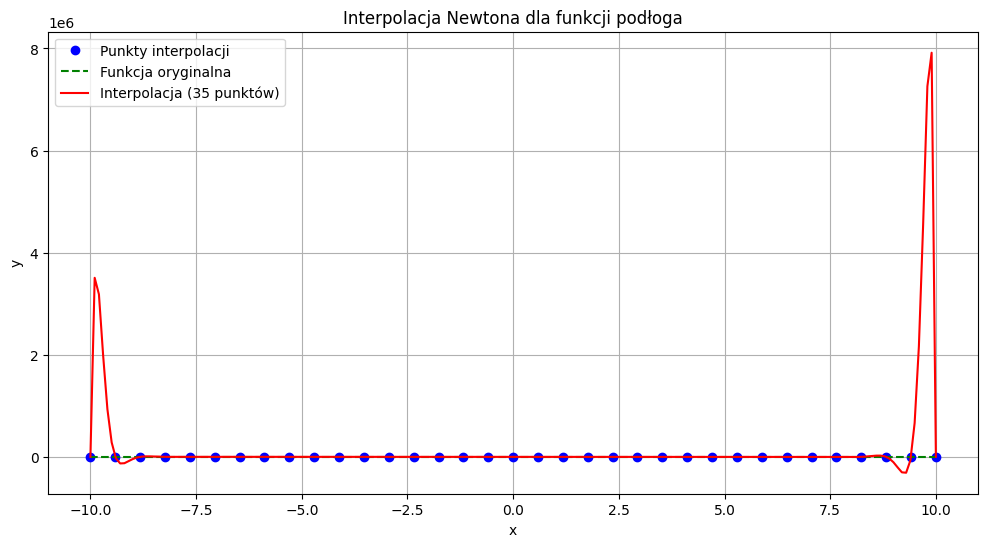
\includegraphics[width=\textwidth]{figures/task-3/floor_35.png}
\end{minipage}

\textbf{Conclusions:}
\begin{itemize}
    \item \textbf{Efficiency with a moderate number of points:} Adding many interpolation points does not necessarily improve results. It can instead increase errors as the algorithm fits a polynomial requiring abrupt changes in function values.
    \item \textbf{Difficulty with discontinuous functions:} Discontinuous functions, such as \( \lfloor x \rfloor \), produce much larger errors because a continuous polynomial cannot fit discontinuities well.
    \item \textbf{Uniformly continuous functions:} Trigonometric and rational functions give better results, although accuracy limitations remain.
    \item Functions with many extrema show characteristic jumps caused by frequent changes in their rate of growth.
\end{itemize}
